\chapter{Implementacija i korisničko sučelje}
		
		
		\section{Korištene tehnologije i alati}
			
			%\textbf{\textit{dio 2. revizije}}
			
			 %\textit{Detaljno navesti sve tehnologije i alate koji su primijenjeni pri izradi dokumentacije i aplikacije. Ukratko ih opisati, te navesti njihovo značenje i mjesto primjene. Za svaki navedeni alat i tehnologiju je potrebno \textbf{navesti internet poveznicu} gdje se mogu preuzeti ili više saznati o njima}.
			
			Frontend aplikacije pisan je u programskom jeziku \textbf{\href{https://www.javascript.com/}{JavaScript}} uz pomoć biblioteke \textbf{\href{https://reactjs.org/}{React}}. React je  open-source JavaScript biblioteka za izgradnju komponenti korisničkog sučelja te je odgovorna samo za prezentacijski sloj aplikacije. Glavni cilj Reacta je razvoj korisničkog sučelja koje poboljšava brzinu aplikacija, pa stoga koristi virtualni DOM (Document Object Model) koji je brži od običnog DOM-a. Aplikacije pisane u Reactu su jednostranične što također pridonosi brzini. Korištenjem komponenti u Reactu, poboljšava se čitljivost i olakšava se održavanje većih aplikacija. React je razvijen od strane Facebooka te korišten i u njihovim aplikacijama poput Instagrama i WhatsAppa.\\
			Kao razvojno okruženje za frontend aplikacije korišten je \textbf{\href{https://code.visualstudio.com/}{Visual Studio Code}}. Visual Studio Code je lagan, ali moćan uređivač izvornog koda razvijen od strane tvrtke Microsoft. Neke od glavnih značajki alata su podrška za ispravljanje pogrešaka, isticanje sintakse, inteligentno dovršavanje koda i mnoge druge. Dolazi s ugrađenom podrškom za JavaScript, TypeScript i Node.js, a ima i bogat ekosustav proširenja za druge jezike i okruženja kao što su C++, C\#, Java, Python, PHP, Go, .NET itd.\\
			Backend aplikacije pisan je u programskom jeziku \textbf{\href{https://www.java.com/en/}{Java}} uz pomoć radnog okvira \textbf{\href{https://spring.io/projects/spring-boot}{Spring Boot}}. Spring Boot je vrlo popularan radni okvir za izgradnju samostojećih aplikacija koje koriste Spring. Spring Boot je specijalizacija radnog okvira Spring razvijen s ciljem jednostavnijeg i bržeg oblikovanja web aplikacija, pa stoga u svojoj automatskoj konfiguraciji olakšava posao programeru jer neke stvari, kao npr. servleti, rad s JSON datotekama, rad s bazama podataka itd., koje su karakteristične za većinu web aplikacja ima automatski podešeno. \\
			Kao razvojno okruženje za backend aplikacije korišten je \textbf{\href{https://www.jetbrains.com/idea/}{IntelliJ IDEA}}. IntelliJ IDEA je integrirano razvojno okruženje (IDE) razvijeno od strane tvrtke JetBrains. Samo razvojno okruženje pisano je u Javi s ciljem poboljšanog razvoja softvera u jezicima Java, Kotlin, Groovy i sl. Ovaj IDE pruža značajke kao što su dovršavanje koda analizom konteksta, navigacija u kodu pri čemu je moguće izravno skakanje na klasu ili deklaraciju u kodu, refaktoriranje koda, otklanjanje pogrešaka i brojne druge. IntelliJ IDEA također podržava dodatke pomoću kojih se može ostvariti dodatna funkcionalnost. Dodaci se mogu preuzeti i instalirati putem njihovog web repozitorija dodataka ili putem IDE-ove ugrađene opcije instaliranja dodataka.\\
			Baza podataka je izvedena u \textbf{\href{https://www.postgresql.org/}{PostgreSQL-u}}. PostgreSQL je open-source sustav za upravljanje relacijskim bazama podataka (RDBMS) kojim se proširuje funkcionalnost SQL-a. PostgreSQL nudi transakcije s okidačima, stranim ključevima, pohranjenim procedurama, automatski ažuriranim prikazima i sl. Transakcije također imaju svojstva atomarnosti, konzistentnosti, izolacije i izdržljivosti (ACID). PostgreSQL dizajniran je da izdrži različita radna opterećenja, od pojedinačnih računa-la, pa sve do skladišta podataka ili web usluga s mnogo istodobnih korisnika. \\
			Kao okruženje za upravljanje bazom podataka korišten je \textbf{\href{https://www.pgadmin.org/}{pgAdmin}}. pgAdmin je open-source grafički alat za administrativno upravljanje PostgreSQL bazama podataka.\\
			Sama dokumentacija je pisana u jeziku \textbf{\href{https://www.latex-project.org/}{LaTeX}}. LaTeX je jezik za pisanje strukturiranih tekstova profesionalne kvalitete. Za razliku od nekih programa za obradu teksta s grafičkim sučeljem poput Microsoft Worda, dokumenti se u LaTeXu pišu kao običan tekst s dodanom semantičkom strukturom te se time postiže usredotočenost na sadržaj, ujednačenost izgleda te brži i stabilniji rad.\\
			Kao okruženje za pisanje dokumentaciju korišten je \textbf{\href{https://www.texstudio.org/}{TeXstudio}}. TeXstudio je open-source integrirano okruženje za izradu LaTeX dokumenata. Posjeduje brojne znač-ajke kao što su pogled na strukturu dokumenta, napredno isticanje sintakse, interaktivna provjera pravopisa, gramatike i referenci, jasan pogled na upozorenja i greške u dokumentu itd.\\
			Za izradu UML dijagrama unutar dokumentacije korišteno je okruženje \textbf{\href{https://astah.net/products/astah-uml/}{Astah UML}}. Astah UML je grafički alat koji je jednostavan za rukovanje te se koristi za izradu potrebnih UML dijagrama. Ima podršku za stvaranje brojnih dijagrama, a samo neki od njih su dijagrami obrazaca uporabe, sekvencijski dijagrami, dijagrami razreda, dijagrami stanja, dijagrami aktivnosti, dijagrami komponenti te dijagrami razmještaja za čiju je izradu alat i korišten.\\
			Za izradu dijagrama baze podataka unutar dokumentacije korišten je online alat \textbf{\href{https://drawsql.app/}{DrawSQL}}.\\
			Kao sustav za upravljanje verzijama projekta korišten je \textbf{\href{https://git-scm.com/}{Git}}. Git je open-source distribuirani sustav za upravljanje različitim verzijama datoteka. Obično se koristi za koordinaciju rada među programerima koji zajednički razvijaju neki softver. Cilj Gita je brzina, integritet podataka i podrška za distribuirane i nelinearne tijekove rada. Svaki Git direktorij na bilo kojem računalu je spremište s potpunom poviješću i punim mogućnostima praćenja verzija.\\
			Udaljeni repozitorij projekta dostupan je na web platformi u oblaku \textbf{\href{https://gitlab.com/}{GitLab}}. GitLab je open-source end-to-end platforma u oblaku za razvoj softvera s ugrađenom kontrolom verzija, praćenjem problema, pregledom koda, CI/CD-om i više.\\
			Za deploy aplikacije korišten je \textbf{\href{https://render.com/}{Render}}. Render je objedinjeni sustav u oblaku koji služi za izgradnju i pokretanje web aplikacija i aplikacija općenito. Pruža pogodnosti poput besplatnih TLS (Transport Layer Security) certifikata, globalnog CDN-a (Content Delivery Network), DDoS (Distributed Denial of Service) zaštite, privatnih mreža i automatske implementacije iz Gita.\\
			Za komunikaciju u timu korišten je \textbf{\href{https://discord.com/}{Discord}}. Discord je društvena platforma na kojoj korisnici imaju mogućnost komuniciranja glasovnim pozivima, videopozivima, tekstualnim porukama, medijima i datotekama u privatnim razgovorima ili kao dio zajednica koje se nazivaju serveri. Server je skup soba za razgovor i glasovnih kanala te mu je moguće pristupiti putem pozivnice.\\
			
			
			\eject 
		
	
		\section{Ispitivanje programskog rješenja}
			
			\textbf{\textit{dio 2. revizije}}\\
			
			 \textit{U ovom poglavlju je potrebno opisati provedbu ispitivanja implementiranih funkcionalnosti na razini komponenti i na razini cijelog sustava s prikazom odabranih ispitnih slučajeva. Studenti trebaju ispitati temeljnu funkcionalnost i rubne uvjete.}
	
			
			\subsection{Ispitivanje komponenti}
			\textit{Potrebno je provesti ispitivanje jedinica (engl. unit testing) nad razredima koji implementiraju temeljne funkcionalnosti. Razraditi \textbf{minimalno 6 ispitnih slučajeva} u kojima će se ispitati redovni slučajevi, rubni uvjeti te izazivanje pogreške (engl. exception throwing). Poželjno je stvoriti i ispitni slučaj koji koristi funkcionalnosti koje nisu implementirane. Potrebno je priložiti izvorni kôd svih ispitnih slučajeva te prikaz rezultata izvođenja ispita u razvojnom okruženju (prolaz/pad ispita). }
			
			
			
			\subsection{Ispitivanje sustava}
			
			 \textit{Potrebno je provesti i opisati ispitivanje sustava koristeći radni okvir Selenium\footnote{\url{https://www.seleniumhq.org/}}. Razraditi \textbf{minimalno 4 ispitna slučaja} u kojima će se ispitati redovni slučajevi, rubni uvjeti te poziv funkcionalnosti koja nije implementirana/izaziva pogrešku kako bi se vidjelo na koji način sustav reagira kada nešto nije u potpunosti ostvareno. Ispitni slučaj se treba sastojati od ulaza (npr. korisničko ime i lozinka), očekivanog izlaza ili rezultata, koraka ispitivanja i dobivenog izlaza ili rezultata.\\ }
			 
			 \textit{Izradu ispitnih slučajeva pomoću radnog okvira Selenium moguće je provesti pomoću jednog od sljedeća dva alata:}
			 \begin{itemize}
			 	\item \textit{dodatak za preglednik \textbf{Selenium IDE} - snimanje korisnikovih akcija radi automatskog ponavljanja ispita	}
			 	\item \textit{\textbf{Selenium WebDriver} - podrška za pisanje ispita u jezicima Java, C\#, PHP koristeći posebno programsko sučelje.}
			 \end{itemize}
		 	\textit{Detalji o korištenju alata Selenium bit će prikazani na posebnom predavanju tijekom semestra.}
			
			\eject 
		
		
		\section{Dijagram razmještaja}
			
			%\textbf{\textit{dio 2. revizije}}
			
			 %\textit{Potrebno je umetnuti \textbf{specifikacijski} dijagram razmještaja i opisati ga. Moguće je umjesto specifikacijskog dijagrama razmještaja umetnuti dijagram razmještaja instanci, pod uvjetom da taj dijagram bolje opisuje neki važniji dio sustava.}
			 
			 Dijagram razmještaja identificira fizičke i virtualne čvorove koji su prisutni u topologiji sustava te opisuje programsku potporu u implementaciji sustava. Sam sustav baziran je na odnosu klijent-poslužitelj + HTTP protokol za komunikaciju između njih. Cijela poslužiteljska strana ostvarena je pomoću servisa Render.
			 
			 \begin{figure}[H]
			 	\centering
			 	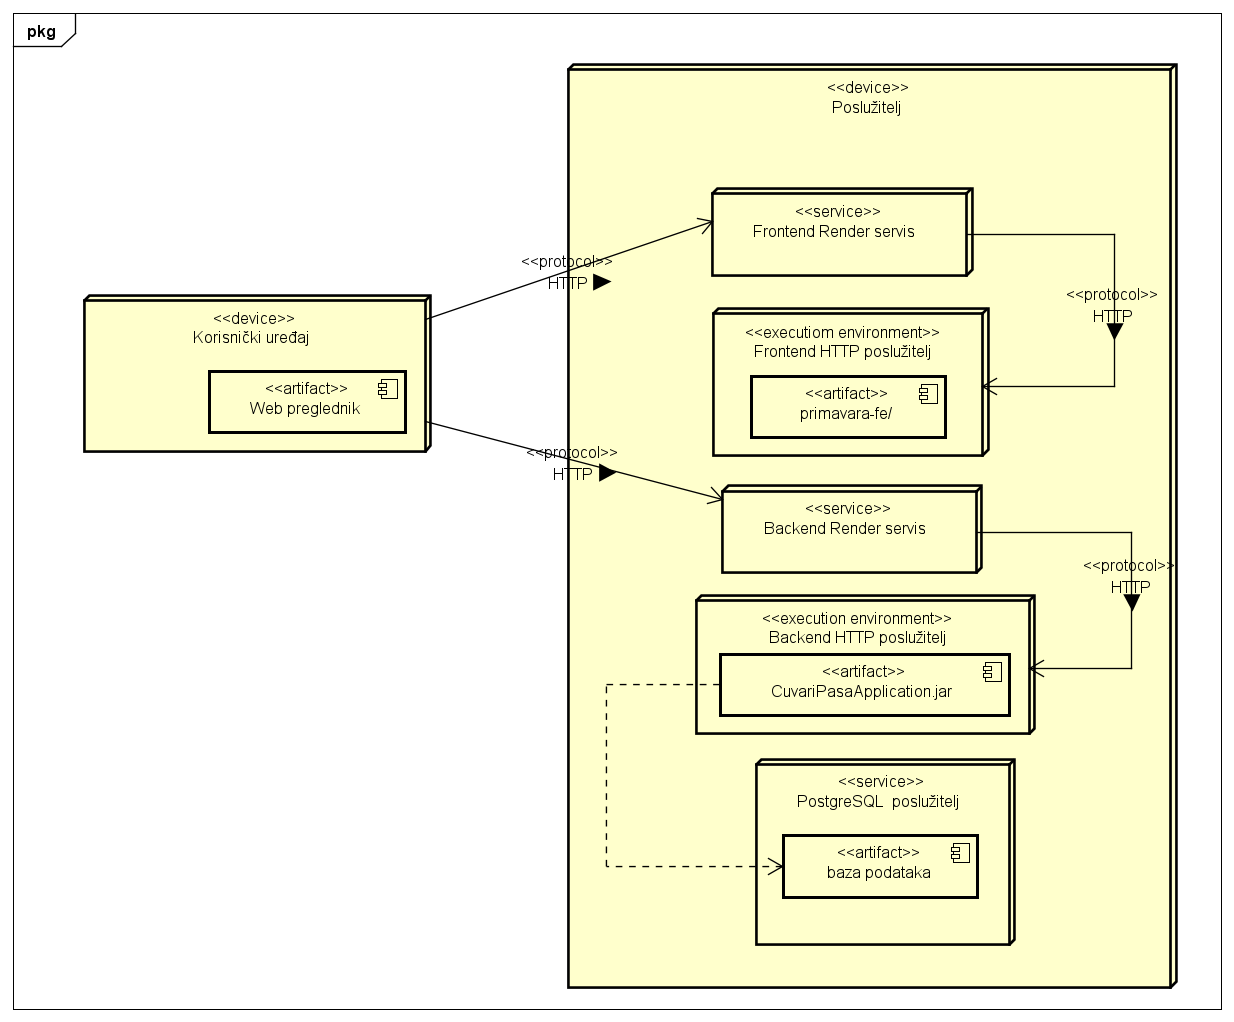
\includegraphics[width=15cm]{slike/Dijagram razmjestaja}
			 	\caption{Dijagram razmještaja}
			 	\label{fig:Activity-Diagram}
			 \end{figure}
			
			\eject 
		
		\section{Upute za puštanje u pogon}
			
			\subsection{Konfiguracija poslužitelja baze podataka}
			
			Na poslužitelju Render potrebno je konfigurirati PostgreSQL bazu podataka. Potrebno je postaviti ime baze, korisničko ime korisnika baze, regiju postaviti na Frankfurt (EU Central) i kliknuti Create Database. Pri prvom pokretanju backenda, automatski će se kreirati svi elementi baze Flyway migracijama.
			
			\begin{figure}[H]
				\centering
				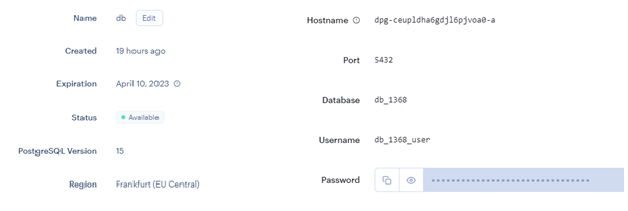
\includegraphics[width=12cm]{slike/konfiguracijaBazeNaRenderu}
				\caption{Konfiguracija baze na Renderu}
				\label{fig:Baza-Render}
			\end{figure}
			
			\subsection{Konfiguracija backenda}
			
			
			Na poslužitelju Render potrebno je konfigurirati backend. Potrebno je povezati GitLab račun s Renderom. Nakon toga potrebno je kreirati novi servis i odabrati projekt Čuvari pasa. Za regiju je potrebno odabrati Frankfurt (EU Central), za granu main, za root directory primavara-be. Environment je potrebno postaviti na Docker. Dockerfile Path je ./docker/maven/Dockerfile, a Docker Build Context Directory je . Potrebno je postaviti environment varijable sa slike 5.3 i nakon toga kliknuti Create Web Service.
			
			\begin{figure}[H]
				\centering
				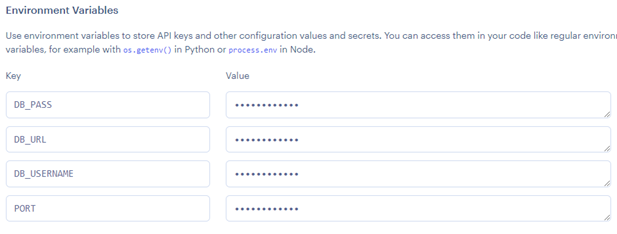
\includegraphics[width=12cm]{slike/konfiguracijaBackenda}
				\caption{Konfiguracija backenda na Renderu}
				\label{fig:Backend-Render}
			\end{figure}
			
			\subsection{Konfiguracija frontenda}
			
			
			Na poslužitelju Render potrebno je konfigurirati frontend. Potrebno je povezati GitLab račun s Renderom. Nakon toga potrebno je kreirati novi servis i odabrati projekt Čuvari pasa. Za regiju je potrebno odabrati Frankfurt (EU Central), za granu main, za root directory primavara-fe. Environment je potrebno postaviti na Node. Build command je potrebno postaviti na yarn build, a start command na yarn start-prod. Potrebno je postaviti environment varijable sa slike 5.4 i nakon toga kliknuti Create Web Service.
			
			\begin{figure}[H]
				\centering
				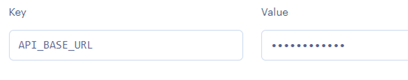
\includegraphics[width=12cm]{slike/konfiguracijaFrontenda}
				\caption{Konfiguracija frontenda na Renderu}
				\label{fig:Frontend-Render}
			\end{figure}
			\eject 